\section{Dinamica}

\subsection{Principi fondamentali}

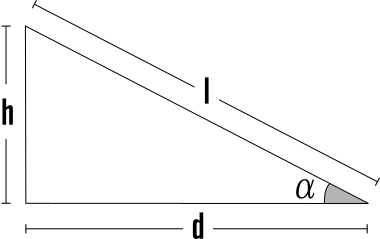
\includegraphics[width=0.4\linewidth]{Dinamica/piano-inclinato-senza-angolo.png} \\

\begin{gather*}
\text{Secondo principio: }
\begin{cases}
    \vec{F} = m \vec{a} \\
    \vec{a} = \frac{\vec{F}}{m} \\
    m = \frac{\vec{F}}{a}
\end{cases} \\
\text{Terzo principio: } \vec{F}_{AB} = -\vec{F}_{BA} \\
\text{$\alpha$(altezza, lunghezza): }\sin{\alpha} = \frac{h}{l} \\ 
\text{$\alpha$(base, lunghezza): }\cos{\alpha} = \frac{d}{l} \\
\text{$\alpha$(altezza, base): }\tan{\alpha} = \frac{h}{d} \\
\end{gather*}
\subsection{Piano inclinato}
\begin{gather*}
    F_{P, x} = F_P \sin (\alpha) = m g \sin (\alpha) \\
    F_{P, y} = F_P \cos (\alpha) = m g \cos (\alpha) 
\end{gather*}
%%%
\subsubsection{Piano inclinato senza attrito}
Piano inclinato: \\
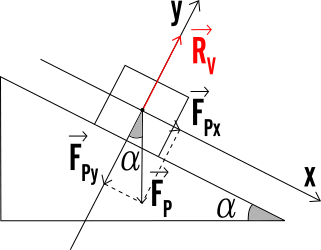
\includegraphics[width=0.75 \linewidth]{Dinamica/reazione-vincolare-nel-piano-inclinato.png} \\
\begin{gather*}
\text{Accelerazione}: \begin{cases}
    a_y = 0 \\
    a_x = g \sin{\alpha}
\end{cases}
\end{gather*}

\subsubsection{Piano inclinato con F verso l'alto}
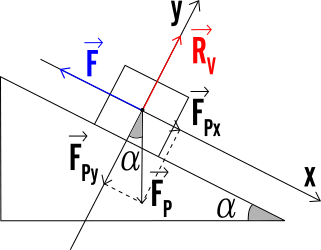
\includegraphics[width=0.75 \linewidth]{Dinamica/variante-piano-inclinato-senza-attrito.png} \\
\textbf{Nota bene: } sull'asse y la forza($F$)che spinge l'oggetto verso l'alto non fa cambiare niente. Ricordiamo che abbiamo scelto \textbf{il piano inclinato} come asse del nostro sistema di riferimento.
\begin{gather*}
    \text{Forza risultante: } F_{ris} = F_{P, x} - F \\
    \text{Accelerazione: } a = \frac{F_{ris}}{m} \\
    \begin{cases}
        F_{P, x} > F & \text{Corpo scende, $a$ positiva} \\
        F_{P, x} < F & \text{Corpo sale, $a$ negativa}
    \end{cases}
\end{gather*}
%%%
\subsubsection{Piano inclinato con attrito}
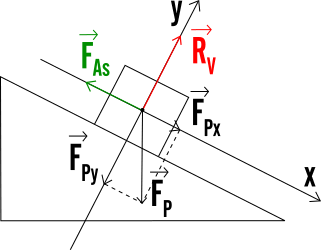
\includegraphics[width=0.75 \linewidth]{Dinamica/piano-inclinato-con-attrito.png} \\
\begin{gather*}
    \text{Forza risultante: } F_{ris, x} = \sqrt{F_{P, x}^2 + F_{As}^2}
\end{gather*}
\textbf{Nota bene: } la forza d'attrito ($F_{A}$, attrito statico nell'immagine) ha verso opposto alla componente della forza peso sull'asse x($F_{P, x}$)
\subsubsection{Attrito Statico}
\begin{gather*}
    \text{Forza Attrito Statico: } \\ F_{As} = \mu_s \cdot F_\perp = \mu_s \cdot F_{P, y} = \mu_s m g \cos (\alpha) \\
    \text{Accelerazione: } \\ a = a_x = g \sin (\alpha) - \mu_s g \cos (\alpha) \\
    \text{Angolo critico per l'equilibrio: } \\ \alpha = \arctan (\mu_s)
\end{gather*}
\subsubsection{Attrito Dinamico}
\textbf{Nota bene: } Per poter considerare il problema dal punto di vista dell'attrito dinamico($\mu_d$)
\begin{gather*}
    \text{Accelerazione: } \\ a = a_x = g \sin (\alpha) - \mu_d g \cos (\alpha)
\end{gather*}